\chapter{Conducteurs et isolants}\label{ch:g4:conductors-insulators}

Pourquoi les fils électriques sont-ils en métal --- mais habillés de
plastique~? Pourquoi le petit pont de l'\omterm{ex:g3:first-electric-circuit:switch}{interrupteur} laisse-t-il
passer le courant, alors que son boîtier garde tes doigts en
sécurité~? L'an dernier, nous fermions des boucles~; cette année,
nous demandons quelles matières l'électricité peut traverser. La
réponse range toutes les matières en deux catégories~: les
\omterm{def:g4:conductors-insulators:conductor}{conducteurs} et les \omterm{def:g4:conductors-insulators:insulator}{isolants}.

\section{Le testeur}

\begin{method}[Construire un testeur]\label{met:g4:conductors-insulators:tester}
Construis la boucle de l'an dernier --- \omterm{def:g3:first-electric-circuit:battery}{pile}, fils, lampe --- mais en
laissant une coupure volontaire~: deux extrémités de fil libres,
écartées d'une largeur de doigt.
\begin{enumerate}
  \item mettre les deux extrémités libres en contact~: la lampe
        s'allume --- le testeur fonctionne~;
  \item combler la coupure avec l'objet à l'essai, une extrémité
        métallique pressée fermement contre chaque fil~;
  \item observer la lampe~: allumée, l'électricité a traversé
        l'objet~; éteinte, elle n'a pas pu.
\end{enumerate}
La lampe donne la réponse~: elle s'allume exactement quand l'objet
testé complète la boucle.
\end{method}

\begin{omfigure}
\begin{tikzpicture}[scale=0.9]
  \draw (0,0) to[battery1, l=pile] (0,2.6)
    to[short] (2.2,2.6)
    to[lamp, l=lampe] (4.4,2.6)
    to[short] (6.0,2.6) -- (6.0,1.7);
  \draw (6.0,0.9) -- (6.0,0) to[short] (0,0);
  \fill (6.0,1.7) circle (1.6pt) node[right, font=\small]
    {~extrémité libre};
  \fill (6.0,0.9) circle (1.6pt) node[right, font=\small]
    {~extrémité libre};
  \draw[thick, fill=omMeth, fill opacity=0.4]
    (5.75,0.95) rectangle (6.25,1.65);
  \node[right, font=\small] at (6.6,1.3) {objet testé};
\end{tikzpicture}

{\small Le testeur~: une boucle en bon état avec une seule coupure.
Ce qui comble la coupure est l'objet à l'essai --- la lampe montre si
le courant le traverse.}
\end{omfigure}

\section{Conducteurs et isolants}

\begin{definition}[Conducteur]\label{def:g4:conductors-insulators:conductor}
Un \emph{conducteur}\index{conducteur} est une matière qui laisse
l'électricité la traverser. Dans le testeur, un conducteur qui comble
la coupure ferme la boucle et allume la lampe.
\end{definition}

\begin{definition}[Isolant]\label{def:g4:conductors-insulators:insulator}
Un \emph{isolant}\index{isolant} est une matière qui bloque
l'électricité. Combler la coupure avec un isolant laisse la boucle
aussi ouverte qu'avant~: la lampe reste éteinte.
\end{definition}

\begin{example}[Une matinée d'essais]\label{ex:g4:conductors-insulators:trials}
Résultats d'un testeur de classe~: un trombone en acier ---
allumée. Une pièce de monnaie --- allumée. Du papier d'aluminium ---
allumée. Une clé --- allumée. Une règle en plastique --- éteinte. Un
crayon en bois --- éteinte. Une bille de verre --- éteinte. Une gomme
en caoutchouc --- éteinte. Une bande de papier --- éteinte. La
régularité saute aux yeux~: les objets qui allument la lampe sont
tous en métal.
\end{example}

\begin{proposition}[Les métaux conduisent]\label{prop:g4:conductors-insulators:metals}
Tous les métaux conduisent l'électricité --- le fer, le cuivre,
l'aluminium, l'or, tous sans exception, ce qui explique que les
caprices de l'\omterm{def:g1:magnets:magnet}{aimant} pour le fer nous aient surpris alors que le
testeur, lui, ne nous surprendra jamais. La plupart des autres
\omterm{def:g3:solids-liquids-gases:solid}{solides} de tous les jours --- plastique, bois, verre, caoutchouc,
papier, cire --- sont des \omterm{def:g4:conductors-insulators:insulator}{isolants}.
\end{proposition}

\begin{remark}[Conducteur ne veut pas dire
magnétique]\label{rem:g4:conductors-insulators:notmagnet}
Ne confonds pas les deux talents des métaux. L'\omterm{def:g1:magnets:magnet}{aimant} ne choisit que
le fer et sa famille~; le courant électrique est bien moins
difficile et traverse \emph{tous} les métaux. Le papier d'aluminium
qui ignorait ton \omterm{def:g1:magnets:magnet}{aimant} conduit le courant à merveille --- deux jeux
différents, deux règles différentes.
\end{remark}

\section{Conducteurs et isolants travaillent ensemble}

\begin{example}[Anatomie d'un fil]\label{ex:g4:conductors-insulators:wire}
Regarde l'extrémité du câble d'une lampe, là où il entre dans la
fiche~: à l'intérieur court du cuivre brillant --- un \omterm{def:g4:conductors-insulators:conductor}{conducteur}, la
route du courant~; tout autour s'enroule du plastique coloré --- un
\omterm{def:g4:conductors-insulators:insulator}{isolant}, la clôture de la route. Le cuivre fait le travail~; le
plastique garde le courant dedans et tes doigts dehors. Tous les
câbles de ta maison associent les deux~: un \omterm{def:g4:conductors-insulators:conductor}{conducteur} à l'intérieur
d'un \omterm{def:g4:conductors-insulators:insulator}{isolant}.
\end{example}

\begin{omfigure}
\begin{tikzpicture}[scale=0.85]
  \draw[thick, fill=omExo, fill opacity=0.25]
    (0.5,0.35) rectangle (6.5,1.65);
  \draw[thick, fill=omThm, fill opacity=0.45]
    (0.5,0.78) rectangle (7.6,1.22);
  \node[right, font=\small] at (8.35,1.8) {gaine de plastique~: isolant};
  \draw[-Stealth, omExo] (8.3,1.8) -- (6.3,1.55);
  \node[right, font=\small] at (8.35,1.0) {âme de cuivre~: conducteur};
  \draw[-Stealth, omExo] (8.3,1.0) -- (7.72,1.0);
\end{tikzpicture}

{\small Un câble électrique déshabillé~: une route de cuivre pour le
courant, à l'intérieur d'une clôture de plastique pour la sécurité.}
\end{omfigure}

\begin{omfigure}
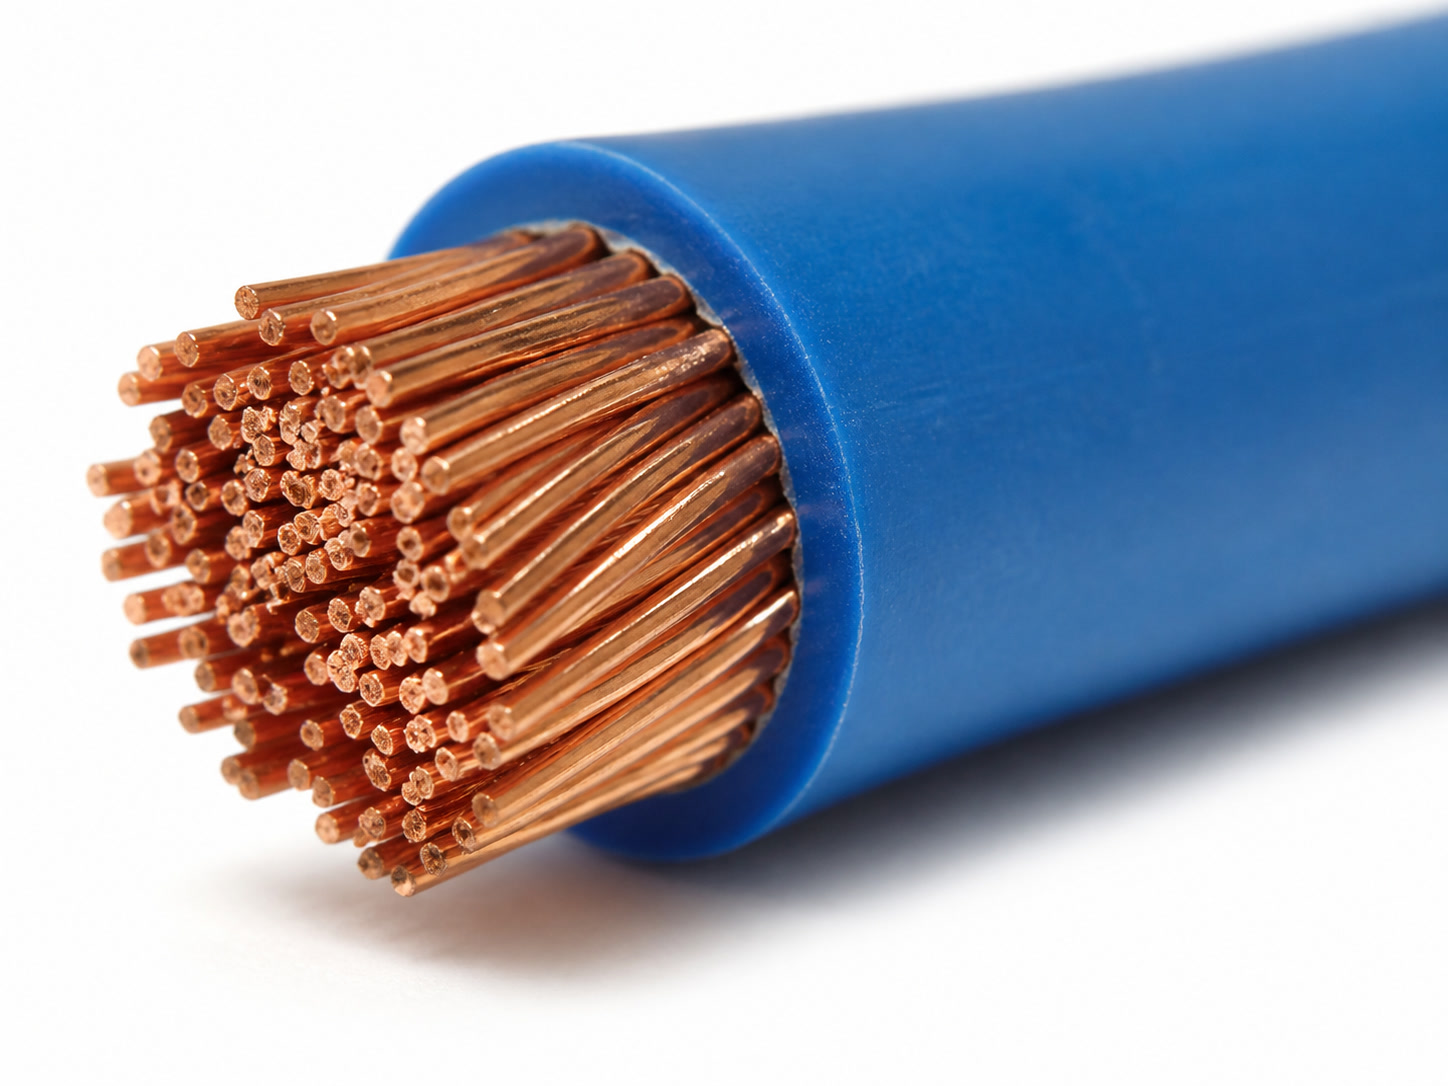
\includegraphics[width=0.5\linewidth]{images/book1/ai/g4-conductors-cable.jpg}

{\small L'extrémité coupée d'un câble, en vrai~: des brins de cuivre brillants --- le \omterm{def:g4:conductors-insulators:conductor}{conducteur} --- à l'intérieur de leur gaine de plastique colorée --- l'\omterm{def:g4:conductors-insulators:insulator}{isolant}.}
\end{omfigure}

\begin{example}[Lire les objets de tous les
jours]\label{ex:g4:conductors-insulators:objects}
Beaucoup d'objets s'expliquent maintenant tout seuls.
L'\omterm{ex:g3:first-electric-circuit:switch}{interrupteur}~: un pont de métal (il doit porter le courant) dans un
boîtier de plastique (ton doigt, lui, ne doit pas). Le tournevis de
l'électricien~: lame d'acier, manche \omterm{def:g4:conductors-insulators:insulator}{isolant} épais. La prise~: du
métal bien au fond, du plastique en façade. Les pylônes portent des
câbles de métal nus, hauts et hors d'atteinte, suspendus à de longs
disques \omterm{def:g4:conductors-insulators:insulator}{isolants} pour que le courant ne fuie pas dans le pylône.
\end{example}

\begin{remark}[L'eau, les humains, et la raison des
règles]\label{rem:g4:conductors-insulators:safety}
Il reste un \omterm{def:g4:conductors-insulators:conductor}{conducteur} à nommer~: les \emph{objets humides} --- y
compris la peau humaine humide. Nous conduisons mal, mais la prise de
courant pousse si puissamment que «~mal~» suffit largement. Voilà la
raison profonde des règles de sécurité que tu connais~: ne jamais
mettre les doigts dans une prise, ne jamais toucher un appareil
électrique avec les mains mouillées, tenir les sèche-cheveux loin de
la baignoire. Le testeur à \omterm{def:g3:first-electric-circuit:battery}{pile} est sans danger \emph{parce que} la
poussée d'une \omterm{def:g3:first-electric-circuit:battery}{pile} est minuscule~; la prise, elle, ne pardonne rien.
\end{remark}

\section{Exercices}

\begin{exercise}[$\star$]\label{exo:g4:conductors-insulators:1}
Qu'est-ce qu'un \omterm{def:g4:conductors-insulators:conductor}{conducteur}~? Un \omterm{def:g4:conductors-insulators:insulator}{isolant}~? Lequel des deux allume la
lampe du testeur~?
\end{exercise}

\begin{exercise}[$\star$]\label{exo:g4:conductors-insulators:2}
Range en \omterm{def:g4:conductors-insulators:conductor}{conducteurs} et \omterm{def:g4:conductors-insulators:insulator}{isolants}~: une cuillère en acier~; \ un
bouchon de liège~; \ du papier d'aluminium~; \ un verre~; \ une pièce
en cuivre~; \ une brique de plastique.
\end{exercise}

\begin{exercise}[$\star$]\label{exo:g4:conductors-insulators:3}
Avant tout essai, comment vérifier que le testeur lui-même
fonctionne~? Pourquoi cette vérification est-elle importante~?
\end{exercise}

\begin{exercise}[$\star$]\label{exo:g4:conductors-insulators:4}
Un objet à l'essai laisse la lampe éteinte. Donne deux raisons
possibles --- l'une au sujet de l'objet, l'autre au sujet d'un essai
mal fait.
\end{exercise}

\begin{exercise}[$\star$]\label{exo:g4:conductors-insulators:5}
Pourquoi le câble d'une lampe est-il en cuivre à l'intérieur et en
plastique à l'extérieur~? Quel métier fait chaque matière~?
\end{exercise}

\begin{exercise}[$\star$]\label{exo:g4:conductors-insulators:6}
Dans un \omterm{ex:g3:first-electric-circuit:switch}{interrupteur}, quelle partie est conductrice et laquelle est
isolante~? Pourquoi a-t-il besoin des deux~?
\end{exercise}

\begin{exercise}[$\star$]\label{exo:g4:conductors-insulators:7}
Le papier d'aluminium ignore complètement un \omterm{def:g1:magnets:magnet}{aimant}. Allumera-t-il la
lampe du testeur~? Quelle règle répond, et contre quelle confusion
\cref{rem:g4:conductors-insulators:notmagnet} met-elle en garde~?
\end{exercise}

\begin{exercise}[$\star$]\label{exo:g4:conductors-insulators:8}
Un crayon, c'est du bois avec une mine de graphite. Le testeur de
Nino reste éteint à travers le bois verni, mais s'allume faiblement
d'une pointe à l'autre en passant par le graphite taillé aux deux
bouts. Qu'a découvert Nino sur les deux matières du crayon~?
\end{exercise}

\begin{exercise}[$\star$]\label{exo:g4:conductors-insulators:9}
Pourquoi les tournevis et les pinces des électriciens ont-ils
d'épais manches en plastique~? Quelle matière protège qui~?
\end{exercise}

\begin{exercise}[$\star\star$]\label{exo:g4:conductors-insulators:10}
Une chaîne de collier donne «~allumée~» dans le testeur~; un collier
de perles en bois donne «~éteinte~»~; un collier de perles de métal
nouées sur un gros fil de coton donne «~éteinte~» aussi --- alors que
chaque perle conduit~! Explique le troisième résultat en suivant la
route du courant, de perle en perle.
\end{exercise}

\begin{exercise}[$\star\star$]\label{exo:g4:conductors-insulators:11}
Pourquoi est-il bien plus dangereux de toucher des appareils
électriques avec les mains mouillées qu'avec les mains sèches~? Et
pourquoi le testeur à \omterm{def:g3:first-electric-circuit:battery}{pile} est-il sans danger pour tes expériences
alors que la prise ne l'est jamais~? Sers-toi de
\cref{rem:g4:conductors-insulators:safety}.
\end{exercise}
